\documentclass{article}
\usepackage[T1]{fontenc}
\usepackage{lmodern}
\usepackage{graphicx}
\usepackage{amsmath,amssymb}
\usepackage[a4paper,margin=2cm]{geometry}
\usepackage[absolute,overlay]{textpos}
\setlength{\TPHorizModule}{1mm}
\setlength{\TPVertModule}{1mm}
\usepackage[indonesian]{babel}
\usepackage{hyperref}
\setlength{\emergencystretch}{2em}
% unit: Halaman 17

\begin{document}

% === Halaman 17 (llm) ===

\vspace{162.16mm}

Giovanni Battista Porta menggambarkan cara menyembunyikan pesan di dalam telur rebus.\\
\nCaranya, pesan ditulis pada kulit telur yang dibuat dari tinta khusus yang dibuat dengan satu ons tawas dan setengah liter cuka.\\
\nPrinsipnya penyembunyiannya adalah tinta tersebut akan menembus kulit telur yang berpori, tanpa meninggalkan jejak yang terlihat.\\
\vspace{10mm}
Giovanni Battista Porta \\ (1535-1615) \\
\vspace{5mm}
Tulisan dari tinta akan membekas pada permukaan isi telur yang telah mengeras (karena sudah direbus sebelumnya). Pesan dibaca dengan membuang kulit telur

% deskripsi: Potret ilustrasi Giovanni Battista Porta dalam bingkai oval.
% bbox normalisasi: [0.0840, 0.0900, 0.3700, 0.6360]
\begin{textblock*}{60.06mm}(17.64mm,26.73mm)
\noindent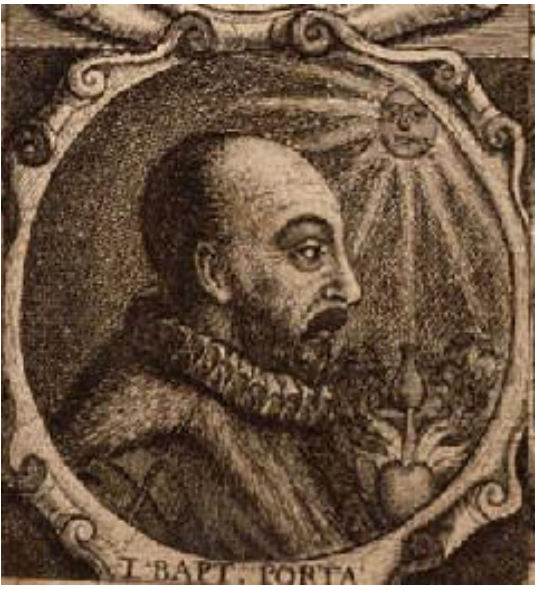
\includegraphics[width=60.06mm,height=162.16mm]{../../images/llm/page_017_img_01.png}%
\end{textblock*}

\end{document}
